\documentclass[12pt]{article}

\usepackage{graphicx}
\usepackage{amsmath}
\usepackage{amsfonts}
\usepackage{apacite}
\usepackage{natbib} 
\usepackage{url}
\usepackage[hidelinks]{hyperref}
\usepackage{cleveref}
\usepackage[utf8]{inputenc}
\usepackage{setspace}
\usepackage{caption}
\usepackage{verbatim}
\usepackage{placeins}
\usepackage{subfigure}
\usepackage{dsfont}
\usepackage{accents}
\usepackage{appendix} % For enhanced appendix formatting
\usepackage[disable]{todonotes}%[disable]
\usepackage{amsthm,empheq}
\usepackage{booktabs} 


\onehalfspacing
\newtheorem{theorem}{Theorem}

\newcommand{\jsh}[1]{\todo[inline,color=green!20, caption={2do}]{\textbf{Jack:}\\#1}}
\crefname{section}{Appendix}{Appendices} % Custom naming for appendices

\title{Insights into the prior to posterior transition through Wasserstein
distances and the power posterior}
\author{Damian Mingo, Jack S. Hale}
\date{\today}

\usepackage{glossaries}

\newacronym{wim}{WIM}{Wasserstein Impact Measure}  
\newacronym{nuts}{NUTS}{No-U-Turn sampler}  
\newacronym{swim}{sWIM}{prior scaled Wasserstein Impact Measure}  
\newacronym{bf}{BF}{Bayes factor}
\newacronym{mcmc}{MCMC}{Markov Chain Monte Carlo}
\newacronym{ott}{OTT}{Optimal Transport Tools}
\newacronym{tfp}{TFP}{Tensorflow Probability}
\newacronym{kl}{KL}{Kullback–Leibler}


\begin{document}


\maketitle


\begin{abstract}

This study investigates how priors transition to posteriors. We analyse this transition by calculating the Wasserstein distance between the priors and the power posteriors. Power posteriors are obtained by raising the likelihood function to values between zero and one, forming a continuous path from the prior to the full posterior. Additionally, we have introduced the concept of saturation sample size and illustrated that it can
be used to reduce the sample size in various studies. The saturation sample size is the number of observations that contain the same amount of information as the entire dataset. Thus, the saturated sample size is important when it is challenging to have larger sample sizes, such as in clinical trials involving rare diseases or when individuals are reluctant to participate in a survey.

\end{abstract}

\section{Introduction}

\jsh{JSH TODO: Opening paragraph - similar to paper 2}

\jsh{JSH TODO: Narrow in on WIM. Measures distances between posteriors which are prior +
data (via likelihood). Explain what the WIM doesn't do.}

\jsh{JSH: TODO: Discuss new idea. Examine the continuous transition between prior and
posterior via the likelihood.}

Priors are a crucial element of Bayesian analysis, and the choices made can significantly impact parameter inference. Various methods have been developed to assess the impact of priors, one of which is the \gls{wim} \citep{ghaderinezhadWassersteinImpactMeasure2022}. The \gls{wim} is the Wasserstein distance between two posteriors resulting from two different priors for a given data set. The \gls{wim} is a relative measure of impact between standard posteriors. However, the methods of prior impact assessment, including the \gls{wim}, do not tell us how the priors transition to the posterior.

Moreover, the \gls{wim} has limitations in its interpretability; for instance, a value of 2.0 does not indicate whether one prior has a higher or lower impact than the other. To illustrate, consider a scenario where the \gls{wim} value is 2.0 for two different priors. This value alone does not provide information on which prior has a higher impact, making it difficult to interpret the results. With theses limitations, there is a need to understand how priors impact inference. Also, to how to set up priors that have minimal influence on the posterior. 

This study employs power posteriors and Wasserstein distances to gain insights into prior to posterior transitions. Power posteriors have been used in many applications, such as calculating the marginal  likelihood \citep{friel2008marginal} and calculating the objective \gls{bf} \citep{ohaganPropertiesIntrinsicFractional1997}, where they are referred to as fractional posteriors. They have also been applied to sample across multimodal distributions and are used to set up power priors \citep{Dimitris_2015, Joseph_2000} for robust Bayesian inference  \citep{Jeffrey_2019}. For conjugate cases, we derive and make use of analytic power posteriors. We use graphs to illustrate how the priors transition to the posteriors.  


The sample size is critical for inference. However, it might be difficult to have large sample sizes for some studies. Fortunately, some sample sizes can give the same amount of information as large sample sizes. Thus, linking sample sizes and power posteriors and saturation sample sizes is essential. 

\subsection{Contribution}
The main contributions of this paper are as follows. Using the concept of the power posterior we construct a continuous family of posteriors between prior and posterior by raising the usual likelihood to a power posterior constant $\gamma \in [0, 1]$. To give a visual intuition of this transition, posterior density plots of the power posteriors living between a prior say uniform prior and the standard posterior for a parameter can be made.

\begin{comment}
\begin{figure}
\begin{center}
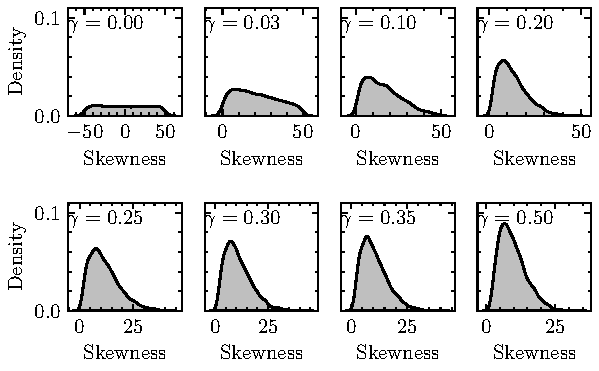
\includegraphics{imgs/uniform_pow.pdf}
\end{center}
\caption{Marginal posteriors for the skewness parameter show the transition
	from a uniform prior ($\gamma=0$) to various power posteriors
	($0 < \gamma \leq 0.5$). Posterior based on the frontier data set for the
	skew-normal distribution.}\label{fig:skew_normal_powpos}
\end{figure}
\end{comment}
From the definition of the power posterior we derive extensions of three
standard conjugate results, namely the Normal-Normal, Normal-Inverse-Gamma and
Poisson-Gamma cases. These conjugate results show that for an observed data set
of size $n$ the product $\gamma n$ as the effective sample size of the observed
data, that is, $\gamma$ can be used to reduce the sample size of the data from
$n$ to $n\gamma$. 

With the definition of the power posterior in hand we then observe the
evolution of the Wasserstein distance between power posterior measures
$\mu_{\gamma}$ and the fixed prior measure $\mu_{0}$. These plots typically show a sudden change in the Wasserstein distance as $\gamma$ is increased just beyond zero (the prior is moved a large distance by a small effective sample size of the data). As $\gamma$ is increased at some point the distance `saturates' and increasing $\gamma$ further (i.e. increasing the effective sample size) does not lead to the posterior moving significantly further away from the prior. This saturation region gives us an indication of a saturated sample size, that is, at which adding more data into the problem (implicitly
via the parameter $\gamma$) does not lead to an increase in the distance
between the power posterior and the prior.  A formal definition of the saturated sample size is the effective sample size at which 

\begin{comment}
\[W_t = CrI \cdot W_{\mu_0,\gamma_1}\]
The saturated sample size is then given by:
\[m_{sat}=\gamma_{W_t​}\cdot n\]
where $\gamma_{W_t​}$  is the $\gamma$ at which $W_t$ becomes constant.
\end{comment}
The saturated sample size $m_{\text{sat}}$ is the total sample size $n$ scaled by the value of $\gamma$ at which the Wasserstein distance between the prior and the standard posterior becomes constant. The scaling factor, $W_t$, is computed as the product of the credible interval ($\text{CrI}$) and the Wasserstein distance between the prior and the standard posterior $W_{\mu_0, \gamma_1}$.

\[
W_t = \text{CrI} \cdot W_{\mu_0, \gamma_1}
\]
The saturated sample size is then given by:
\[
m_{\text{sat}} = \gamma_{W_t} \cdot n
\]
where $\gamma_{W_t}$ is the $\gamma$ at which $W_t$ becomes constant.


We demonstrate through simulations that subsampling is equivalent to power posteriors, where the power $\gamma$ serves as a weight for the data, resulting in a reduced sample size.

In addition to looking at an prior to posterior transition for a single fixed prior, we also look at the evolution of the Wasserstein distance under different prior assumptions with the findings illustrated in graphs. 

\section{Methodology}

This section covers the concepts and methodologies used in this study, such as power posteriors, Wasserstein distance calculations, subsampling, and numerical methods. We make use of conjugate cases where the power posteriors are available in closed. 
	
\subsection{Power posterior}
We briefly recall the mathematical concept of the power posterior (sometimes
also called the fractional posterior) which is central to this paper. Let $x$
be some observed data and $p(x\, | \, \theta)$ be the likelihood function of a
model that depends on a set of parameters $\theta$ with associated prior
$p(\theta)$. Moreover, let $\gamma$ be an additional \emph{power posterior
constant} in the interval $[0, 1]$. Then the power posterior
\citep{friel2008marginal} can be defined as
\begin{equation}
\label{eq:pow_pos}
p(\theta \, | \, x,\gamma) := \frac{p(x \, | \, \theta)^\gamma p(\theta)}{z}, \quad \gamma \in [0, 1],
\end{equation}
where $z := p(x)$ is a normalising constant called the marginal likelihood. It
is straightforward to see that for $\gamma = 0$ we recover the usual Bayesian
prior $p(\theta)$ and for $\gamma = 1$ we recover the standard Bayesian
posterior $p(\theta \, | y)$. We emphasise that for intermediate values $\gamma
\in (0, 1)$ the resulting set of power posteriors forms a continuous
transition between the standard prior and posterior distribution. The likelihood  $p(x|\theta)$ reflects how likely it is for a parameter to generate the data. If we take the $\log$ of $p(x \, | \, \theta)^\gamma$ we can see from $\gamma \log p(x|\theta)$ that $\gamma$ 
controls the relative weight of the log-likelihood (and consequently the data) with respect to the log-prior.

\subsection{Wasserstein distance}
Various measures are used to quantify the discrepancies between distributions. These measures involve computing the  \gls{kl} and chi-square divergence. However, these divergences \citep{aliGeneralClassCoefficients1966} are not symmetric, and even when symmetric versions exist, other challenges arise. For instance, the \gls{kl} divergence is undefined if the intersection of the support of the two distributions in question is a null set. In contrast, Wasserstein distance is symmetric, can be computed between discrete and continuous probability distributions, considers the geometry of the parameter space \citep{panaretos2019statistical}, and is a well-defined metric. Therefore, we employ the Wasserstein distance.
The definition of the $p$-Wasserstein distance ($W_p$) between two probability
measures $\mu, \nu$ defined on the space $\mathcal{X}$  is 
\begin{equation}
W_p(\mu, \nu) = \inf_{\pi \in U(\mu, \nu)} \left(\int_{\mathcal{X} \times \mathcal{X}}||x-y||^pd\pi(x, y) \right)^{1/p}, \quad p\geq 1,
\label{wasser:ana1}
\end{equation}
where $U(\mu, \nu)$ is the set of joint probability measures on
$\mathcal{X}\times \mathcal{X}$ \citep{villaniOptimalTransportOld2009}, $x$ and $y$ are points in the space $X$. The
Wasserstein distance has a natural interpretation as the minimum amount of work
required to reconfigure the mass of one distribution into another.

\begin{comment}
 Calculating
the Wasserstein distance becomes non-trivial in moderate to high dimensions due
to the ill-posed nature of the squared Euclidean distance
\citep{cuturiMongeBregmanOccam2023}. 
\end{comment}

\subsection{Subsampling}
Subsampling refers to the method of drawing a random sample from a dataset to analyse it as a representative of the complete dataset \citep{Drineas_2006, yaoReviewOptimalSubsampling2021, Ma_2014}. Consider $\{x_i\}_{i=1}^n$ are $n$ independent and identically distributed observations. We can draw a subsample of size $m$ from the entire sample of size $n$ with sampling probabilities $\{\pi_i\}_{i=1}^n$ on each observation. The observations have equal sampling probabilities. The motivation for subsampling is to avoid the computational expense of analysing the entire data set. 

Subsampling is similar to using power posteriors. When working with large datasets, using power posteriors with a power value close to 1 can be a practical strategy to manage computational complexity and reduce the impact of model misspecification. To demonstrate this, we calculated the expectation of the Wasserstein distance between the priors and the standard posterior across multiple subsamples of size $m= \gamma n$, where $m$ is the subsample size, $n$ is the size of the entire dataset, and $\gamma$ varies for each subsample. We also calculated the Wasserstein distances between the priors and their corresponding power posteriors. This enables us to compare the Wasserstein distance between the prior and the standard posterior with respect to subsampling and the Wasserstein distance between the prior and the power posteriors.

\begin{comment}
We found that the expectation of the Wasserstein distance between the prior and the standard posterior with respect to subsampling converges to the same value as the Wasserstein distance between the priors and the power posteriors.
\end{comment}
\subsection{Posterior measures}
In this section, we introduce several measures that will be important in the results section. The first measure is the prior distribution, $\mu_0$, representing our initial beliefs or assumptions before analysing any data. Next, we have the power posterior, $\mu_{\gamma}$, which is a variation of the standard posterior that raises the likelihood to a constant $\gamma$, ranging from 0 to 1, to adjust the influence of the data on inference. Another key measure is the squared 2-Wasserstein distance between the power posterior and the prior distribution $W_2^2(\mu_{\gamma}, \mu_0)$. Moreover, we define the expectation of 
this squared 2-Wasserstein distance between a standard posterior $\mu_1$ and the prior $\mu_0$ as the average of these distances across multiple subsamples from the dataset. This expectation is calculated as  \begin{equation}
	E [W_2^2(\mu_1, \mu_0)] = \frac{1}{S}\sum_{i=1}^{S} W_2^2(\mu_1, \mu_0),
	\label{eq:wasser_ex}
\end{equation}
where $S$ represents the number of subsamples, each of size $m$, drawn from the full dataset of size $n$. 
 
\subsection{Numerical methods}
We give a brief overview of the numerical methods used to generate the results.
For full details see the references provided below.

Samples from the power posteriors and priors are generated using \gls{mcmc},
specifically the \gls{nuts} \citep{hoffman2014}. We use the version implemented
within \gls{tfp} \citep{dillonTensorFlowDistributions2017} running on the JAX
backend \citep{jax2018github}.

We remark that exploring power posteriors within \gls{tfp} is straightforward
and only requires the programmatic definition of the log power-posterior. This
involves scaling the provided log-likelihood evaluation by $\gamma$ and then
adding the log-prior terms. This can be achieved in a few lines of code and the
resulting function passed to any of the \gls{mcmc} methods built-in to
\gls{tfp}.

The skew-normal distribution is not implemented in \gls{tfp}, so we wrote a
custom distribution using Distrax \citep{deepmind2020jax} following the
numerical methodology described in \citep{ghorbanzadeh_method_2014}. 

To calculate Wasserstein-1 distance for the one-dimensional problems we use the
Vallender formula \cite{vallender_calculation_1974} which relates the
1-Wasserstein distance between two probability measures $\mu_1$ and $\mu_2$ on
$\mathbb{R}$ with cumulative distribution functions $F_1(x)$ and $F_2(x)$,
respectively
\begin{equation}
W_1(\mu_1, \mu_2) = \int_{\mathbb{R}} | F_1(x) - F_2(x) | \; \mathrm{d}x.
\end{equation}
We approximate the Vallender formula using the dedicated function available in
SciPy \citep{2020SciPy-NMeth}. 

For the multi-dimensional case we cannot use to the Vallender formula to
compute the Wasserstein distance. Instead we use recent advances in
computational optimal transport to estimate the Wasserstein distance.
Specifically, we use entropic regularised optimal transport proposed in
\citep{NIPS2013_af21d0c9} and its implementation within the \gls{ott} library
\citep{cuturi2022optimal}. 


All code and data used to produce the results in this paper will be available
as supplementary material upon journal submission.

\section{Summary of methodology}
This section gives a concise overview of the methodology.  We employ conjugate cases where the power posteriors are available in closed. A conjugate case occurs when the prior and the posterior distributions are of the same family. We formally introduce the concept of saturation sample size, which links subsampling to power posteriors. The connection is demonstrated by subsampling with different sample sizes. 

\subsection{Evolution of the Wasserstein distances}
\begin{enumerate}
	\item Generate data from the models. This step is necessary since we use synthetic data, and the step is not required if observed data is available.
	\item Set up different priors and a likelihood function. Obtain the power posteriors. For conjugate cases, the power posteriors are available in closed form. 
	\item Compute the Wasserstein distances between the priors and their corresponding power posteriors. The Wasserstein distance is available in closed form for a normal prior and a normal likelihood function. 
\end{enumerate}

\subsection{Subsampling}

\begin{enumerate}
	\item Set up a sequence of $\gamma$ values from 0 to 1. For each value of $\gamma$, compute the Wasserstein distances between the priors and the power posteriors using the entire dataset. 
	\item For each value of $\gamma$, draw $S$ subsamples, each of size $m$ from the entire dataset, where \[m=\gamma n,\] with $\gamma \in [0, 1]$ representing the power, and $n$ is the sample size of the entire data set.
	\item For each subsample, compute the Wasserstein distances between the priors and the respective standard posteriors.
	\item Compute the expectation of the Wasserstein distances across the $S$ subsamples.
	\item Also, take note of the saturation sample size.
\end{enumerate}
	The saturation sample size is the number of observations needed to achieve a value of $\gamma$ at which the Wasserstein distance between the power posterior and the prior reaches $95\%$ or $99\%$ of the Wasserstein distance between the full posterior ($\gamma=1$) and the prior($\gamma=0$). In other words, the saturation sample size is the number of observations required to reach a critical value of $\gamma$. This critical value of $\gamma$ tells us the power posterior or the number of observations needed to construct the full posterior.



\section{Results}
This section presents the results of the transition of various priors to their corresponding posteriors. These results are based on experiments with power posteriors for conjugate cases and a skew-normal distribution. Also, we illustrate that subsampling yields results equivalent to those obtained through power posteriors.
\subsection{Normal-normal conjugate case with unknown mean}
Following standard arguments, it is possible to show that the distribution of
the power posterior for the following Bayesian model with dataset $x = (x_1,
\ldots, x_n)$
\begin{subequations}
\begin{align}
x_1, \ldots, x_n &\overset{\mathrm{iid}}{\sim} \mathcal{N}(m, \sigma^2), \\
m &\sim \mathcal{N}(m_0, \sigma_0^2),
\end{align}
\end{subequations}
is normally distributed (see \cref{appen}, \cref{proof:pow_norm} for proof)
\begin{equation*}
m \;|\; \bar{x}, \gamma \sim \mathcal{N} \left( \left( \frac{1}{\sigma_0^2} + \frac{\gamma n}{\sigma^2} \right)^{-1} \left(\frac{m_0}{\sigma_0^2} + \frac{\gamma n \bar{x}}{\sigma^2}  \right), \left( \frac{1}{\sigma_0^2} + \frac{\gamma n}{\sigma^2} \right)^{-1} \right),
\end{equation*}
where $\bar{x} = (\sum x_i)/ n$ is the sample mean. We remark that, as
expected, the prior is recovered when $\gamma = 0$ and the classic
normal-normal with unknown mean conjugate result is recovered when $\gamma =
1$. The role of $\gamma$ in this context is to reduce the contribution of each
element of the dataset through the likelihood. More specifically for the
normal-normal case, the effective data set size is reduced from the standard
posterior ($\gamma = 1$) from $n$ to $n \gamma$ in the power posterior. Note
however, regardless of the value of $\gamma > 0$, the entire dataset $x$ is
still used in the update from prior to the power posterior.

The 2-Wasserstein metric ($p = 2$) for two non-degenerate normal
measures $\mu_1$ and $\mu_2$ on $\mathbb{R}$ with means $m_1, m_2 \in
\mathbb{R}$ and variances $\sigma_1^2, \sigma_2^2 \in \mathbb{R}_{>0} :=
\left\lbrace x \in \mathbb{R} \; | \; x > 0 \right\rbrace$, respectively, can
be found in closed form as
\begin{equation*}
W_{2} (\mu_1, \mu_2)^2 = \left( m_1 - m_2 \right)^2 + \sigma_1^2 + \sigma_2^2 - 2 \bigl( \sigma_2 \sigma_1^2 \sigma_2 \bigr)^{1/2}.
\end{equation*}
Consequently in this case there is no need to resort to approximate numerical
computations to compute the Wasserstein metric. In closed form the Wasserstein
metric between the prior measure $\mu_0$ and the measure induced by the power posterior
$\mu_\gamma$ is
\begin{equation*}
W_2(\mu_0, \mu_\gamma)^2 = \sigma_{0}^{2} + \frac{\sigma^{2} \sigma_{0}^{2}}{p} + \frac{\left(\gamma m_{0} n \sigma_{0}^{2} - \gamma n \sigma_{0}^{2} \bar{x}\right)^{2}}{p^{2}} - \frac{2 \sigma \sigma_{0}^{2}}{\sqrt{p}}
\end{equation*}
with $p = \gamma n \sigma_{0}^{2} + \sigma^{2}$.
Letting $\gamma = 0$ it can be verified that $W_2(\mu_0, \mu_0)^2 = 0$. 

In the first experiment we generate a (small) dataset of size $n = 10$ from a
normal distribution with zero mean and unit variance. We propose three prior
choices (\cref{priors_inorm_norm}) by adjusting the prior parameters $m_0$ and $\sigma_0^2$:
\begin{enumerate}
\item \emph{Non-informative prior}.  With
this relatively flat prior we expect the posterior to be `data prominent'
and highly sensitive to the inclusion of information via the likelihood,
here controlled by the parameter $\gamma$.
\item \emph{Informative `correct' prior}.
This prior expresses definite information about the parameter that
coincidentally coincides with the true parameter. 
\item \emph{Informative `incorrect' prior}.
This prior expresses definite information about the parameter that
does not coincide with the true parameter value. 
\end{enumerate}

\begin{table}[h!]
	\caption{Priors and their corresponding distributions the Normal likelihood normal prior case.}
	\renewcommand{\arraystretch}{1.5}
	\centering
	\begin{tabular}{cc}
		\toprule
		Priors   & Distribution \\
		\midrule
		Non informative  &  $\mathcal{N}(0.0, 100) $   \\
				Informative    `correct'  & $\mathcal{N}(0.0, 2)$\\
		Informative `incorrect'  & $\mathcal{N}(-5.0, 2)$    \\
		\bottomrule
	\end{tabular}
	\label{priors_inorm_norm}
\end{table}

In \cref{fig:normal_normal_wasserstein_distance_different_priors} we calculate
the squared 2-Wasserstein distance between the posterior measure $\mu_\gamma$
for varying values of $\gamma$ and under the three prior assumptions just
described. All three distances appear to be monotonically increasing in
$\gamma$. The distance between the posterior and prior as $\gamma \to 1$ is
largest ($\sim10^2$) for the non-informative prior, and smallest ($\sim 1$) for
the informative `correct' prior. For the non-informative prior as $\gamma$ is
increased from $0$ we can see a very sudden increase in the metric, which
supports the intuition that the posterior is `data prominent' or `data
sensitive`. By comparison, the distance for the informative `correct' prior
evolves to its final distance more slowly, reflecting that the information
contained in the prior does not strongly disagree with that in the data. The
informative `incorrect' prior sits in between the two extreme cases.
\begin{figure}
\begin{center}
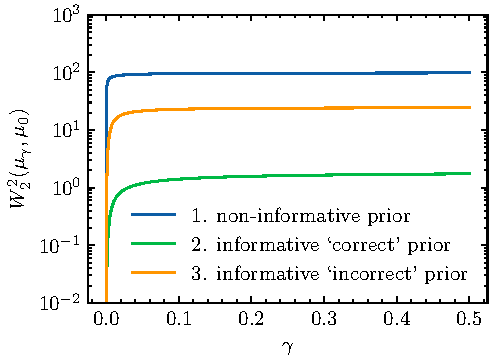
\includegraphics{imgs/normal_normal_wasserstein_distance_different_priors.pdf}
\end{center}
\caption{Normal-normal conjugate case; plot showing squared
2-Wasserstein metric between power posterior and prior against the
power posterior parameter $\gamma \in [0, \frac{1}{2}]$ under the three
different prior assumptions described in the text.}\label{fig:normal_normal_wasserstein_distance_different_priors}
\end{figure}

Given the interpretation of the parameter $\gamma n$ as an effective sample size
in the normal-normal setting, we briefly contrast the power posterior approach
with an approach based on using the standard posterior and varying the size $n$
of the dataset.

To demonstrate the relationship between subsample size and the power posterior, we begin by generating 1000 samples from a standard normal distribution. We then draw 500 subsamples, each of size $m = \gamma n$ where $n = 1000$ and $\gamma$ varies from 0 to 1. For each subsample, we compute the squared 2-Wasserstein distance between the prior and the standard posterior, as well as the mean of these Wasserstein distances, using \cref{eq:wasser_ex}. The results, along with the corresponding $\pm 2\sigma$  interval around the mean, are presented in \cref{fig:normal_normal_compare_with_subsampling}. Additionally, we calculate the squared 2-Wasserstein distance between the prior and the power posterior for various values of $\gamma$. 

In addition, \cref{fig:normal_normal_compare_with_subsampling} illustrates the convergence of the Wasserstein distance 1) between the prior ($\gamma=0$) and the power posteriors $\gamma \in (>0, 1)$ and  2) between the prior and the standard posteriors ($\gamma=1$)  as $\gamma$ increases. As $\gamma$ approaches 1, this convergence exemplifies the increasing similarity between the power and standard posteriors with subsampling. Also, the uncertainty in the standard posterior estimates decreases as $\gamma$ approaches 1, or in other words, as the subsample size increases. For higher values of $\gamma$, the power posteriors and the standard posteriors with subsampling will lead to similar results. 

\begin{figure}[h!]
\begin{center}
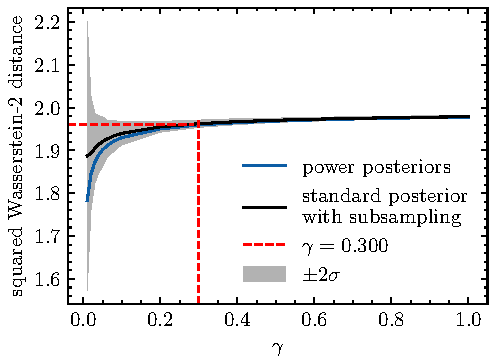
\includegraphics{imgs/sat_samplesize_100_99.pdf}
\end{center}
\caption{Normal-normal conjugate case with unknown mean. Wasserstein distance between the prior and power posteriors compared to the distance between the prior and standard posterior with subsampling. The dashed lines represents the Wasserstein distance and the parameter $\gamma$ at the saturation sample size.}\label{fig:normal_normal_compare_with_subsampling}
\end{figure}

The saturation sample size is also shown in \cref{tab:satsize}. We see that a sample sizes are reduced from 1000 to 300 or 30 depending on the chosen credible interval. By employing the concept of saturation sample size require to get the same information as the total sample size drops. 


\begin{table}[h]
	\caption{Saturation sample size and credible intervals for the Normal prior Normal likelihood case.}
	\renewcommand{\arraystretch}{1.5}
	\centering
		\begin{tabular}{ccccc} 
			\hline
			Wasserstein & $\gamma$ & Saturation & Total & Credible\\
			distance& &sample size& sample size& intervals\\ [0.5ex] 
			\hline 
			1.873 & 0.0300 & 30 & 1000 & 95\%\\
			1.979 & 0.300 & 300 & 1000 & 99\% \\
			\hline
		\end{tabular}
	\label{tab:satsize}
\end{table}
\FloatBarrier
\subsection{Inverse-Gamma conjugate case with unknown variance}
Following standard arguments, it is possible to show that the distribution of
the power posterior for the following Bayesian model with dataset $x = (x_1,
\ldots, x_n)$
\begin{subequations}
\begin{align}
x_1, \ldots, x_n &\overset{\mathrm{iid}}{\sim} \mathcal{N}(m, \sigma^2), \\
\sigma^2 &\sim \text{Inv-Gamma}(\alpha, \beta)
\end{align}
\end{subequations}
with $\alpha, \beta \in \mathbb{R}_{>0}$, is distributed according to an
inverse gamma distribution (see \cref{appen}, \cref{proof:pow_ing} for proof)
\begin{equation*}
\sigma^2 \; | \; s^2, \gamma \sim \text{Inv-Gamma}\left( \alpha + \frac{\gamma n}{2}, \beta + \frac{\gamma n}{2} s^2 \right). 
\end{equation*}
where $s^2 = (\sum_{i} \left( x_i - \mu \right)^2)/n$ is the uncorrected sample
variance. Again, setting $\gamma = 0$ recovers the prior, and setting $\gamma =
1$ recovers the usual conjugate result for the standard Bayesian posterior.

We explore how the Wasserstein distance between the prior and power posteriors changes. Firstly, we generate data of size 100 from a standard normal distribution. Then, an inverse gamma prior with different values of the shape and scale parameters is used, giving three sets of priors (\cref{priors_invg}): informative correct, non-informative prior, and informative incorrect prior.

\begin{table}[h!]
	\caption{Priors and their corresponding distributions.}
	\renewcommand{\arraystretch}{1.5}
	\centering
	\begin{tabular}{cc}
	\toprule
		Priors      & Distribution  \\
		\midrule
		Non informative    &  $\text{Inv-Gamma}(1.0, 1.0)$  \\
		Informative `incorrect'   & $\text{Inv-Gamma}(3.0, 0.5)$    \\
		Informative    `correct'  & $\text{Inv-Gamma}(3.0, \sqrt{2})$\\
		\bottomrule
	\end{tabular}
	\label{priors_invg}
\end{table}

The priors are used to fit three different models to the data with a normal likelihood. For each prior, the Wasserstein distance between the prior and the power posteriors is calculated. When using a non-informative prior, this distance increases with the value of $\gamma$, eventually levels off  at a $\gamma$ value between 0.1 and 0.2 (\cref{fig:ing_conju}). In contrast, the distance decreases initially for informative priors but eventually stabilises. Nonetheless, as $\gamma$ increases, all priors converge to the same distance due to incorporating more data.

\FloatBarrier
\begin{figure}[h]
\begin{center}
        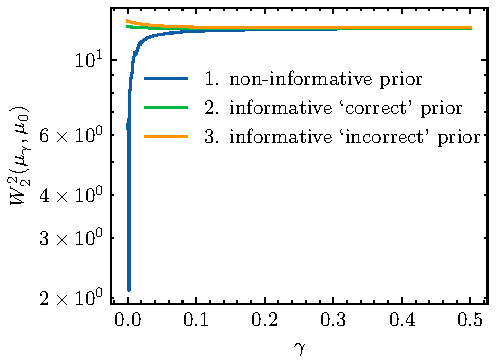
\includegraphics{imgs/inv_gamma_wasserstein_distance.pdf}     
\end{center}
        \caption{Inverse-Gamma conjugate case with unknown variance; plot showing squared
2-Wasserstein metric between power posterior and prior against the
power posterior parameter $\gamma \in [0, \frac{1}{2}]$ under the three
different prior assumptions described in  \cref{priors_invg}.}
    \label{fig:ing_conju}
\end{figure}

\subsection{Poisson-Gamma conjugate case with unknown rate}

The distribution of the power posterior of the following Bayesian model with
dataset $x = (x_1, \ldots, x_n)$ 
\begin{subequations}
\begin{align}
x_1, \ldots, x_n &\overset{\mathrm{iid}}{\sim} \text{Poisson}(\lambda), \\
\lambda &\sim \text{Gamma}(\alpha, \beta),
\end{align}
\end{subequations}
where $\lambda \in \mathbb{R}_{>0}$ is the unknown rate parameter, and $\alpha,
\beta \in \mathbb{R}_{>0}$ are prior parameters is given by (see \cref{appen}, \cref{proof:poisson_gamma} for proof)

\begin{equation}
\lambda \; | \; \bar{x} \sim \text{Gamma} \left( \alpha + \gamma n \bar{x}, \beta + \gamma n \right)
\end{equation}

We investigate the impact of three different sets of priors on the posterior distribution. We generate 100 observations from a Poisson distribution with a rate parameter 1.0. We employ three sets of priors \cref{priors_gammaPois} with a Poisson likelihood for the analysis. 
\begin{table}[h!]
	\caption{Priors and their corresponding distributions.}
	\renewcommand{\arraystretch}{1.5}
	\centering
	\begin{tabular}{cc}
		\toprule
		Priors                   & Distribution\\
		\midrule
		Non informative                    &  $\text{Gamma}(1.0, 1.0)$\\
		Informative `incorrect'         & $\text{Gamma}(10.0, 1.0)$\\
		Informative    `correct'               & $\text{Gamma}(1.0, 0.2)$\\
		\bottomrule
	\end{tabular}
	\label{priors_gammaPois}
\end{table}


We compute the squared Wasserstein distance between each prior and its corresponding power posterior. Our analysis indicates that as $\gamma$ increases, the distance also increases for non-informative priors, while it decreases with increasing $\gamma$ for informative but incorrect priors \cref{fig:poisson_ga_conju}. Eventually, the distances stabilise across all priors. Informative priors converge to the same values, and an elbow point is observed for all priors, beyond which the distance levels off. For the Inverse Gamma prior, this stabilisation occurs just before reaching a value of 0.2.



\begin{figure}[h]
    \begin{center}
   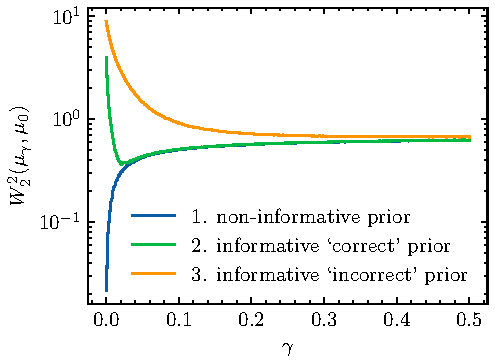
\includegraphics{imgs/poisson_gammawasserstein_distance.pdf}
       \end{center}
        \label{fig:pois_gama_was}
    \caption{Poisson-Gamma conjugate case with unknown rate. Plot showing squared
    	2-Wasserstein metric between power posterior and prior against the
    	power posterior parameter $\gamma \in [0, \frac{1}{2}]$ under the three
    	different prior assumptions described in  \cref{priors_gammaPois}.}
    \label{fig:poisson_ga_conju}
\end{figure}


To further study the relation between sampling and $\gamma$ , we draw 50 subsamples, each of size $m$ where $m =\gamma n$ with $n=100$. We then compute the squared Wasserstein distance between the prior and each subsample for different values of $\gamma$ and then the mean of the Wasserstein distance. Additionally, we calculate the distance between the priors and the power posteriors, and the results are presented in \cref{fig:poisson_ga_conju}. The squared Wasserstein distance converges more rapidly compared to the Normal normal case. The Wasserstein distance converges when $\gamma$ is below 0.2. Similar to the normal normal case, the uncertainty is greatest at lower values of $\gamma$, especially when the subsample size is smaller as shown in  \cref{fig:poisson_gamma_sub}. 


\begin{figure}
\begin{center}
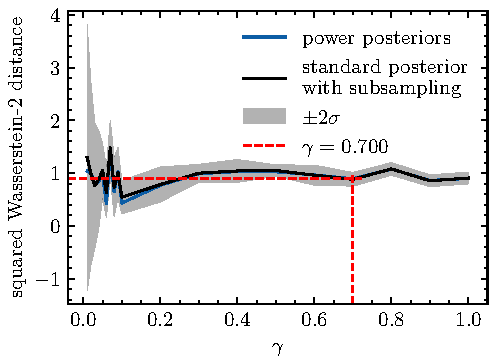
\includegraphics{imgs/poisson_gamma_99.pdf}
\end{center}
\caption{Comparison of the distances for power posteriors and standard posteriors with subsampling. The dashed lines represents the Wasserstein distance and the parameter $\gamma$ at the saturation sample size. Poisson-Gamma conjugate case with unknown rate.}\label{fig:poisson_gamma_sub}
\end{figure}

We also calculated the saturation sample size, which is presented in Table \cref{tab:satsize}. The saturation sample size is reached at \(\gamma\) levels of 0.600 for a 95% credible interval and 0.700 for a 99% credible interval. This indicates that having 60 or 70 observations provides the same amount of information as the entire dataset.

\begin{table}[h]
	\caption{Saturation sample size and credible intervals for the Poisson Gamma model.}
	\renewcommand{\arraystretch}{1.5}
	\centering
	\begin{tabular}{ccccc} 
		\hline
		Wasserstein & $\gamma$ & Saturation & Total & Credible\\
		distance& &sample size& sample size& intervals\\ [0.5ex] 
		\hline 
		0.726 & 0.600 & 60 & 100 & 95\%\\
		0.770 & 0.700 & 70 & 100 & 99\% \\
		\hline
	\end{tabular}
	\label{tab:satsize}
\end{table}

\FloatBarrier
\subsection{Skew-normal distribution}
To gain more insight into prior-to-posterior transitions, we analysed the frontiers data set found in the R package sn  \citep{azzalini2023}. \cite{ghaderinezhadWassersteinImpactMeasure2022} previously analysed this data set. The data set is interesting because the maximum likelihood estimate of the coefficient of skewness lies on the boundary of the range [-0.995, 0.995] acceptable for the skew-normal family. The data was generated by drawing 50 samples from a skew-normal distribution with a skewness parameter 5.0. 
\begin{equation}
    f(x; \alpha) = \frac{2}{\sigma} \phi \left( \frac{x - \mu}{\sigma} \right) \Phi \left( \alpha \frac{(x - \mu)}{\sigma} \right), \quad x \in \mathbb{R}
    \label{skew_n}
\end{equation}
The density of a random variable $x$ that follows a skew-normal distribution \citep{azzaliniClassD1985} is given by \cref{skew_n}.
where $\phi$ is the standard normal probability density function, $\Phi$ is the cumulative distribution function of the standard normal distribution, $\mu$ is the location, $\sigma$ is the scale parameter`n and $\alpha$ is the skewness parameter.
We fit the skew-normal distribution to the data with different sets of priors
for the skewness parameter as in
\cite{ghaderinezhadWassersteinImpactMeasure2022}. We compare the Wasserstein
distance between  power posteriors and the priors. The priors are
Uniform prior, Jeffreys prior, Bayes-Laplace prior,  Beta total variation prior (BTV), normal prior. The squared Wasserstein distance between the priors and the power posteriors
are in \cref{fig:skew_diff_priors}. The distance between
the prior ($\gamma=0$) and the power posteriors increases with an increase in
$\gamma$ but becomes stable as $\gamma$ approaches 1. However, unlike the conjugate cases, the distances do not converge to the same value as the plots are distinguishable.

The priors employed in this section are the same as those in  \citep{ghaderinezhadWassersteinImpactMeasure2022}. What differentiates this study is that we do not compute the \gls{wim}; instead, we compute the Wasserstein distance between the priors and the power posteriors. The aim is to explore the evolution of the Wasserstein distance and how the priors transition to the posteriors for the skew-normal distribution. 

\begin{figure}
\begin{center}
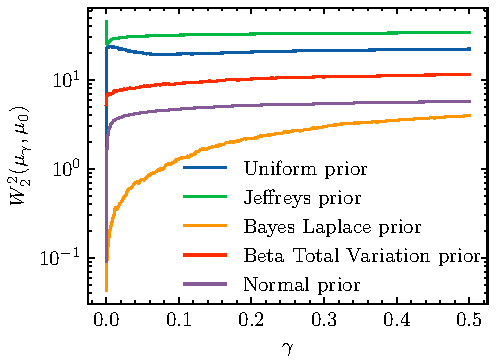
\includegraphics{imgs/wasser_distskew.pdf}
\end{center}`
\caption{Squared Wasserstein distance between the prior and various power
posteriors for different values $\gamma \in [0, 0.5]$ on the frontiers
data set.}\label{fig:skew_diff_priors}
\end{figure}

Another way to visualise prior to posterior transitions  is through density plots  of the priors and the power posteriors. 
\begin{comment}
Plots of the uniform and Jeffreys priors illustrate how the prior density transitions to
the posterior. 
\end{comment}
For the uniform prior \cref{fig:ref_skew_normal_powpos}, the mode is not visible, but as $\gamma$
starts increasing, a mode becomes visible, and the uniform distribution starts
transitioning into a skew distribution. On the other hand, the mode is visible
for Jeffreys prior \cref{fig:skew_jeff_powpos}, but there is no skewness. As $\gamma$ increases, the mode
becomes more visible, and skewness becomes visible. As the value of $\gamma$
increases, the mode becomes more peaked, and the range of the skewness
parameter decreases. When $\gamma=0$, the prior is less informative with no skewness. A $\gamma$ increases, the prior develops a clear peak and becomes right-skewed. Skewness increases with increasing values of $\gamma$. This indicates the prior transitions from a less informative to an informative posterior ( skew normal posterior ) as $\gamma$ increases. Like in the uniform flat prior, as $\gamma$ increases, the prior peaks with less uncertainty and skewness to the right. The density plot of the priors ($\gamma=0$)  \cref{fig:skew_prior} and the standard posteriors ($\gamma=1$) \cref{fig:skew_pos} are shown for comparison with the power posteriors.

\begin{figure}
	\begin{center}
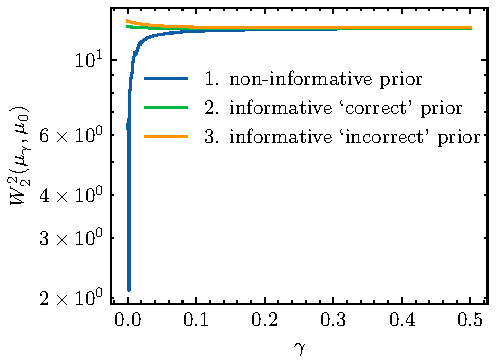
\includegraphics{imgs/inv_gamma_wasserstein_distance.pdf}
\end{center}
\caption{Marginal posteriors for the skewness parameter show the transition
from a uniform prior ($\gamma=0$) to various power posteriors
($0 < \gamma \leq  \frac{1}{2}$). Posterior based on the frontier data set for the
skew-normal distribution.}\label{fig:ref_skew_normal_powpos}
\end{figure}
\begin{figure}
\begin{center}
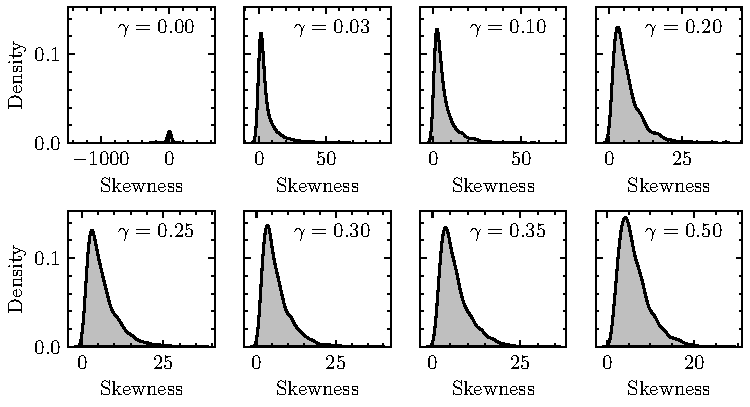
\includegraphics{imgs/Jeffreys.pdf}
\end{center}
\caption{Marginal posteriors for the skewness parameter show the transition
	from Jeffreys prior ($\gamma=0$) to various power posteriors
	($0<\gamma\leq \frac{1}{2}$).  Posterior based on the frontier data set for the
	skew-normal distribution. }\label{fig:skew_jeff_powpos}
\end{figure}
\begin{figure}
	\begin{center}
		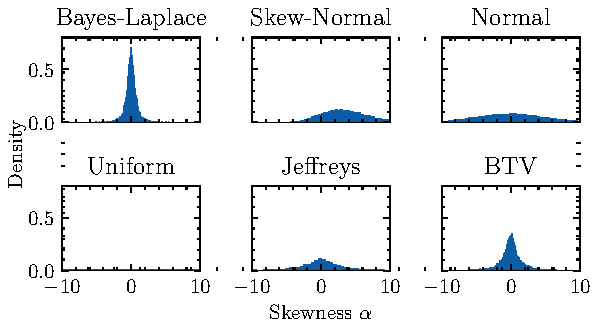
\includegraphics{imgs/prior_histograms1.pdf}
	\end{center}
	\caption{Frontier skew-normal: different priors. Beta total variation prior (BTV)}\label{fig:skew_prior}
\end{figure}
\begin{figure}
	\begin{center}
		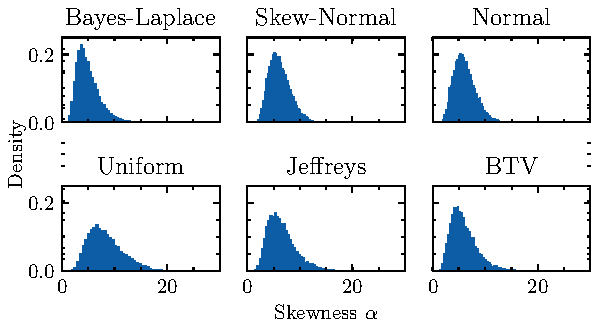
\includegraphics{imgs/posterior_histograms1.pdf}
	\end{center}
	\caption{Frontier skew-normal: posteriors under different priors. These are standard posteriors for the different priors. The posteriors are all positively skewed, unlike the priors in \cref{fig:skew_prior} but with different modes.
	}\label{fig:skew_pos}
\end{figure}

We now explain the importance of the concepts of power posteriors and saturation sample sizes. Power posteriors can be employed to specify prior distributions \citep{ohaganPropertiesIntrinsicFractional1997}. The power posteriors that occur before reaching the saturation sample size can be used to construct weakly informative priors. These priors allow the likelihood to dominate the posterior but still provide minimal information about the parameters. This is because the Wasserstein distance between the prior and the power posteriors is highest at lower values of $\gamma$, implying that at lower values of $\gamma$, the prior has a high influence on the posterior.

Another important application of power posteriors is in determining appropriate sample sizes. For example, in clinical trials, interim analyses are conducted to adapt patient recruitment strategies based on the results of these analyses. One of these strategies is reducing the original sample size or recruiting more patients for a specific treatment arm \cite{Berry2006, Ryan2022}. The saturation sample size can be used to decide if recruiting more patients will make any difference or to stop patient recruitment. This is of enormous importance in the case of rare diseases where patient recruitment is difficult or if there are ethical concerns. The saturation sample size can also inform when to stop recruiting more survey participants.




\FloatBarrier
\section{Conclusion and discussions}
In this study, we explored prior-to-posterior transitions using power posteriors. We have demonstrated that power posteriors weight the sample size, making them similar to subsampling techniques.  The region from $\gamma =0$ to $\gamma =1$ forms a continuous path, transitioning smoothly from the prior distribution to the power posteriors, including the standard posterior. The distance between the prior and the standard posterior increases from $\gamma =0$ to $\gamma =1$. 
The power posterior converges to the standard posterior as the power value increases. For conjugate cases, the posterior distribution stabilises at lower power values, which we confirmed using the Wasserstein distance. Using density plots, we see that the prior transitions to power posteriors closer to the standard posterior at lower $\gamma$ values suggesting that power posteriors can be a good alternative for parameter inference. They are currently used to handle model misspecification \citep{Jeffrey_2019}.

We also provided derivations of power posteriors for conjugate cases.  Additionally, power posteriors can be applied with lower power values to derive data-driven priors. This involves using a part of the data to create these priors and the remainder for the main analysis.

Furthermore, power posteriors allow for the use of improper priors with a subset of the data to derive proper priors, which are then utilised in subsequent analysis. This approach is similar to the fractional \gls{bf} approach proposed by \cite{ohaganPropertiesIntrinsicFractional1997}, where updating an improper prior with a portion of the data helps refine it into a proper prior for the main analysis.

We have also introduced the concept of saturation sample size, which has implications for clinical trials and survey statistics. The saturation sample size is the number of observations with the same amount of information as the entire dataset. This saturation sample size occurs at a $\gamma$ and power posterior. The power posterior corresponding to the value of $\gamma$ at saturation sample size can be used for inference as it provides the same information as the standard posterior. 
It might be difficult to recruit more survey or clinical trial participants. In the case of clinical trials, an interim analysis can be done to determine if the saturation sample size has been reached. For survey statistics, the saturation sample size can be calculated in real time as more participants complete the survey. The study can be concluded once the saturation sample size has been reached.

\section*{Code and data availability}
The complete code used to generate the results will be available in a public repository upon submission.

\section*{Competing interests}
The authors declare no competing interests. 

\section*{Acknowledgements}
This work was funded under the Luxembourg National Research Fund under the
PRIDE programme (PRIDE17/12252781).


%\begin{appendices}
\jsh{These appendices are not referenced in the main text}
\appendix
\section{Appendix}
\subsection{Power posteriors for conjugate cases}\label{appen}
	\begin{theorem}
		\label{proof:pow_norm}
		Let  $m$  be a parameter normally distributed with prior mean $m_0$ and prior variance $\sigma^2_0$. The observed data is $x = (x_1, ..., x_n)$ with sample mean $\bar{x}$ and the data model is $x\overset{\mathrm{iid}}{\sim} \mathcal{N}(m,\sigma^2)$.
		The power posterior can be written
		
		\begin{equation}
			m \;|\; \bar{x}, \gamma \sim \mathcal{N} \left( \left( \frac{1}{\sigma_0^2} + \frac{\gamma n}{\sigma^2} \right)^{-1} \left(\frac{m_0}{\sigma_0^2} + \frac{\gamma n \bar{x}}{\sigma^2}  \right), \left( \frac{1}{\sigma_0^2} + \frac{\gamma n}{\sigma^2} \right)^{-1} \right).\notag
		\end{equation}
		
		\begin{proof}
			The standard posterior $\gamma=1$ is a normal distribution and can be expressed as 
			\begin{equation*}
				m \;|\; \bar{x} \sim \mathcal{N} \left( \left( \frac{1}{\sigma_0^2} + \frac{n}{\sigma^2} \right)^{-1} \left(\frac{m_0}{\sigma_0^2} + \frac{n \bar{x}}{\sigma^2}  \right), \left( \frac{1}{\sigma_0^2} + \frac{n}{\sigma^2} \right)^{-1} \right),
			\end{equation*}
			\cite[see e.g.][]{gelman_bayesian_2020} for proof.
			Taking the normal likelihood and raising it to the power $\gamma$ gives 
			\begin{align}
				p(\bar{x} \;|\ m)^\gamma &\propto \exp\left(-\frac{n}{2\sigma^2}{(\bar{x} - m)^2}\right)^\gamma \notag\\
				& \propto \exp\left(-\frac{\gamma n}{2\sigma^2}{(\bar{x} - m)^2}\right). \notag
			\end{align}
			
			Then, the power posterior can be derived by making the substitution $ \sigma^2 \to \frac{\sigma^2}{\gamma}$ into the standard posterior.
		\end{proof}
	\end{theorem}
	
	\begin{theorem}
		\label{proof:pow_ing}
		Let $m$ be the mean and $\sigma^2$ be the unknown variance. The observed data is denoted as $x = (x_1, ..., x_n)$. The prior variance follows the inverse gamma distribution with shape parameter $\alpha$ and scale parameter $\beta$. The data model is $x\overset{\mathrm{iid}}{\sim} \mathcal{N}(m,\sigma^2)$. The power posterior can be written as
		
		\begin{equation}
			\sigma^2 \;|\; s^2, \gamma \sim \mathrm{IG}\left(\alpha+ \frac{\gamma n}{2}, \beta+\frac{\gamma n}{2}s^2\right),\notag
		\end{equation}
		where, $s^2 = (\sum_{i} \left( x_i - \mu \right)^2)/n$ is the  sample
		variance.
		
		\begin{proof}
			The standard posterior $\gamma=1$ is an inverse gamma and can be expressed as    
			
			\begin{equation*}
				\sigma^2  \;|\; s^2 \sim \mathrm{IG}\left(\alpha + \frac{n}{2}, \beta + \frac{1}{2} \sum(x_i - m)^2 \right),
			\end{equation*}
			\cite[see e.g.][]{gelman_bayesian_2020} for proof.
			Taking the normal likelihood and raising it to the power $\gamma$ gives 
			\begin{equation*}
				p(x_1\ldots,x_n|\sigma^2)^{\gamma}=(\sigma^2)^{-\frac{\gamma n}{2}}\exp\left(-\frac{\gamma}{2\sigma^2}\sum(x_i-m)^2\right).
			\end{equation*}
			This power posterior can be derived by inspection and substituting  $\alpha+ \frac{n}{2} \to \alpha+ \frac{\gamma n}{2}$ and $\beta+\frac{1}{2}\sum(x_i -m)^2 \to \beta+\frac{\gamma}{2}\sum(x_i -m)^2$  in the standard posterior. 
		\end{proof}
	\end{theorem}
	
	\begin{theorem}
		\label{proof:poisson_gamma}
		Let $\lambda$ be the rate parameter of the Poisson distributions, the observed data is $x = (x_1,\ldots, x_n)$ and the data model is $x \overset{\mathrm{iid}}{\sim} \text{Poisson}(\lambda)$. When $\lambda$ has a gamma prior with parameters $\alpha$ and $\beta$, the power posterior can be written as
		
		\begin{equation*}
			\lambda \mid \bar{x} \sim \mathrm{Gamma}\left(\gamma  n \bar{x} + \alpha, \gamma n + \beta\right).
		\end{equation*}
		
		\begin{proof} 
			The standard posterior $\gamma=1$ is a gamma distribution and can be expressed as 
			\begin{align*}
				\lambda \mid  \bar{x} &\sim \text{Gamma}\left( n \bar{x} + \alpha, n + \beta\right)\\
				\bar{x}&=\sum x_i/n,
			\end{align*}
			\cite[see e.g.][]{gelman_bayesian_2020} for proof.
			Raise the likelihood to the power $\gamma$ 
			
			\begin{equation}
				p(x\mid\lambda)^\gamma = \frac{e^{-n \gamma \lambda}\lambda^{\sum x_i}}{\prod_{i=1}^n(x_i !)\gamma}
			\end{equation}
			The power posterior can be derived by substituting 
			$\sum x_i + \alpha \to  \gamma \sum x_i + \alpha$ and  $n + \beta \to  \gamma n + \beta$ in the standard posterior.
		\end{proof}
	\end{theorem}

%\end{appendices}
\bibliographystyle{apacite}
\bibliography{ref}
\end{document}
